\subsection{Linear Solver}

\def \pepoat {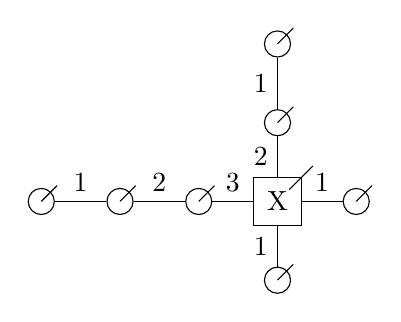
\begin{tikzpicture}[baseline=0.5]

        \def \legLength { 0.8}
        \def \radius {0.1}

        \pgfmathsetmacro{\step}{2*\radius+ \legLength} % 1
        \pgfmathsetmacro{\legpos}{\radius+\legLength} %0.9

        \node[draw,minimum size=0.6cm] (O0) at (0,0) {X};
        \draw (0.15,0.15) -- ++(0.3,0.3);

        \node[draw, circle,radius=\radius] (L1) at (-1,0) {};
        \node[draw, circle,radius=\radius] (L2) at (-2,0) {};
        \node[draw, circle,radius=\radius] (L3) at (-3,0) {};

        \node[draw, circle,radius=\radius] (U1) at (0,1) {};
        \node[draw, circle,radius=\radius] (U2) at (0,2) {};

        \node[draw, circle,radius=\radius] (D1) at (0,-1) {};

        \node[draw, circle,radius=\radius] (R1) at (1,0) {};

        \draw (O0) -- node [above] {3}  (L1);
        \draw (L2) -- node [above] {2}  (L1);
        \draw (L2) -- node [above] {1}  (L3);

        \draw (O0) -- node [left] {2}  (U1);
        \draw (U2) -- node [left] {1}  (U1);

        \draw (O0) -- node [above] {1}  (R1);

        \draw (O0) --  node [left] {1} (D1);

        \draw (L1.center) -- ++(0.2,0.2);
        \draw (L2.center) -- ++(0.2,0.2);
        \draw (L3.center) -- ++(0.2,0.2);
        \draw (U1.center) -- ++(0.2,0.2);
        \draw (U2.center) -- ++(0.2,0.2);
        \draw (R1.center) -- ++(0.2,0.2);
        \draw (D1.center) -- ++(0.2,0.2);

    \end{tikzpicture}}

\def \blockat {  \begin{tikzpicture}[baseline=0.5]

        \def \legLength { 0.8}
        \def \radius {0.1}

        \pgfmathsetmacro{\step}{2*\radius+ \legLength} % 1
        \pgfmathsetmacro{\legpos}{\radius+\legLength} %0.9

        %\node[draw=none] (O0) at (0,0) {};
        \node[draw=none,minimum size=0.6cm] (O0) at (0,0) {B};
        \draw (0.15,0.15) -- ++(0.3,0.3);

        \node[draw=none] (L1) at (-1,0) {};
        \node[draw=none] (L2) at (-2,0) {};
        \node[draw=none] (L3) at (-3,0) {};

        \node[draw=none] (U1) at (0,1) {};
        \node[draw=none] (U2) at (0,2) {};

        \node[draw=none] (D1) at (0,-1) {};

        \node[draw=none] (R1) at (1,0) {};

        %\draw (O0.center) -- ++(0.45,0.45);
        \draw (L1.center) -- ++(0.2,0.2);
        \draw (L2.center) -- ++(0.2,0.2);
        \draw (L3.center) -- ++(0.2,0.2);
        \draw (U1.center) -- ++(0.2,0.2);
        \draw (U2.center) -- ++(0.2,0.2);
        \draw (R1.center) -- ++(0.2,0.2);
        \draw (D1.center) -- ++(0.2,0.2);

        \draw (-3.3,0.3)--(-0.3,0.3) -- (-0.3,2.3)--(0.3,2.3)
        -- (0.3,0.3) -- (1.3,0.3) -- (1.3,-0.3) -- (0.3,-0.3)
        -- (0.3,-1.3) -- (-0.3, -1.3) -- (-0.3,-0.3) -- (-3.3,-0.3) -- cycle;

    \end{tikzpicture}}

\def \pepobt {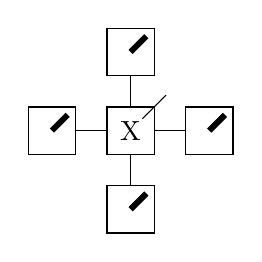
\begin{tikzpicture}[baseline=0.5]

        \def \legLength { 0.8}
        \def \radius {0.1}

        \pgfmathsetmacro{\step}{2*\radius+ \legLength} % 1
        \pgfmathsetmacro{\legpos}{\radius+\legLength} %0.9

        %\node[draw, circle, radius=\radius] (O0) at (0,0) {};
        \node[draw,minimum size=0.6cm] (O0) at (0,0) {X};
        \draw (0.15,0.15) -- ++(0.3,0.3);

        \node[draw, minimum size=0.6cm] (L1) at (-1,0) {};
        \node[draw, minimum size=0.6cm] (U1) at (0,1) {};
        \node[draw, minimum size=0.6cm] (D1) at (0,-1) {};
        \node[draw, minimum size=0.6cm] (R1) at (1,0) {};

        \draw (O0) -- (L1);
        \draw (O0) -- (U1);
        \draw (O0) -- (R1);
        \draw (O0) -- (D1);

        %\draw(O0.center) -- ++(0.2,0.2);
        \draw[line width=0.75mm]  (L1.center) -- ++(0.2,0.2);
        \draw[line width=0.75mm] (U1.center) -- ++(0.2,0.2);
        \draw[line width=0.75mm] (R1.center) -- ++(0.2,0.2);
        \draw[line width=0.75mm] (D1.center) -- ++(0.2,0.2);

    \end{tikzpicture} }

\def \blockbt {   \begin{tikzpicture}[baseline=0.5]

        \def \legLength { 0.8}
        \def \radius {0.1}

        \pgfmathsetmacro{\step}{2*\radius+ \legLength} % 1
        \pgfmathsetmacro{\legpos}{\radius+\legLength} %0.9

        %\node[draw=none] (O0) at (0,0) {};
        \node[draw=none,minimum size=0.6cm] (O0) at (0,0) {B};
        \draw (0.15,0.15) -- ++(0.3,0.3);

        \node[draw=none] (L1) at (-1,0) {};
        \node[draw=none] (L2) at (-2,0) {};
        \node[draw=none] (L3) at (-3,0) {};

        \node[draw=none] (U1) at (0,1) {};
        \node[draw=none] (U2) at (0,2) {};

        \node[draw=none] (D1) at (0,-1) {};

        \node[draw=none] (R1) at (1,0) {};

        %\draw (O0.center) -- ++(0.45,0.45);
        \draw[line width=0.75mm] (L3.center) -- ++(0.2,0.2);
        \draw[line width=0.75mm] (U2.center) -- ++(0.2,0.2);
        \draw[line width=0.75mm] (R1.center) -- ++(0.2,0.2);
        \draw[line width=0.75mm] (D1.center) -- ++(0.2,0.2);

        \draw (-3.3,0.3)--(-0.3,0.3) -- (-0.3,2.3)--(0.3,2.3)
        -- (0.3,0.3) -- (1.3,0.3) -- (1.3,-0.3) -- (0.3,-0.3)
        -- (0.3,-1.3) -- (-0.3, -1.3) -- (-0.3,-0.3) -- (-3.3,-0.3) -- cycle;

    \end{tikzpicture} }

\def \pepoct { 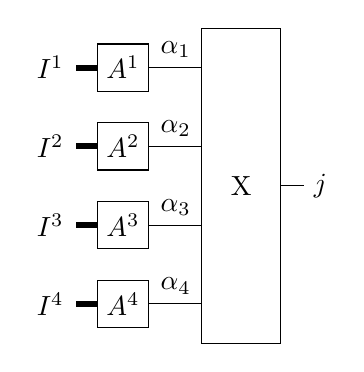
\begin{tikzpicture}[baseline=0.5]
        \draw (0,2.5)-- (0,-1.5) -- (1,-1.5)-- (1,2.5) -- cycle;

        \node[draw=none] (x)  at (0.5,0.5) {X};

        \node[draw, minimum size=0.6cm] (n1)  at (-1,2) {$A^1$};
        \node[draw, minimum size=0.6cm] (n2)  at (-1,1) {$A^2$};
        \node[draw, minimum size=0.6cm] (n3)  at (-1,0) {$A^3$};
        \node[draw, minimum size=0.6cm] (n4)  at (-1,-1) {$A^4$};

        \draw (n1) -- node [above] {$\alpha_1$} (0,2);
        \draw (n2) -- node [above] {$\alpha_2$} (0,1);
        \draw (n3) -- node [above] {$\alpha_3$} (0,0);
        \draw (n4) -- node [above] {$\alpha_4$} (0,-1);

        \draw[line width=0.75mm] (n1) -- ++(-0.6,0) node [left] {$I^1$};
        \draw[line width=0.75mm] (n2) -- ++(-0.6,0) node [left] {$I^2$};
        \draw[line width=0.75mm] (n3) -- ++(-0.6,0) node [left] {$I^3$};
        \draw[line width=0.75mm] (n4) -- ++(-0.6,0) node [left] {$I^4$};

        \draw (1,0.5) -- (1.3,0.5)  node [right] {$j$} ;

    \end{tikzpicture} }

\def \blockct { 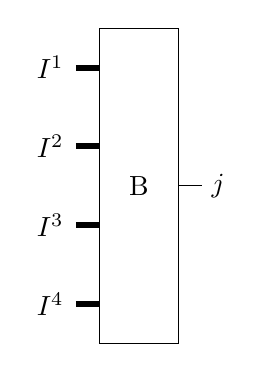
\begin{tikzpicture}[baseline=3]
        \draw (0,2.5)-- (0,-1.5) -- (1,-1.5)-- (1,2.5) -- cycle;

        \node[draw=none] (x)  at (0.5,0.5) {B};

        \draw[line width=0.75mm] (-0.3,2)  node [left] {$I^1$}  -- (0,2) ;
        \draw[line width=0.75mm] (-0.3,1)  node [left] {$I^2$} -- (0,1);
        \draw[line width=0.75mm] (-0.3,0)  node [left] {$I^3$} -- (0,0);
        \draw[line width=0.75mm] (-0.3,-1)  node [left] {$I^4$} -- (0,-1);

        \draw (1,0.5) -- (1.3,0.5)  node [right] {$j$} ;

    \end{tikzpicture} }

\begin{frame}{Linear Solver: Standard Form}
    \begin{equation}
        \only<1>{ \vcenter{\hbox{ \pepob{5}{5}{{
                                "-","-","-","-",
                                "-","-","-","-",
                                "1","2","3","1",
                                "-","-","-","-",
                                "-","-","-","-"}}{{
                                "-","-","-","-",
                                "-","-","-","-",
                                "-","-","-","-",
                                "-","1","2","1",
                                "-","-","-","-"}}{{
                                1,1,1,1,1,
                                1,1,1,0,1,
                                0,0,0,0,0,
                                1,1,1,0,1,
                                1,1,1,0,1}} }} }
        \only<2>{  \pepoat \;  =  \;\blockat  }
        \only<3>{ \pepobt \;  =  \;\blockbt }
        \only<4>{ \vcenter{\hbox{ \pepoct }}  =\vcenter{\hbox{  \blockct }} }
    \end{equation}
\end{frame}

\begin{frame}{Linear Solver: Inversion Scheme}
    \begin{itemize}
        \only<1-> {\item Invert $A^i$ separately }
              \only<1>{
                  \begin{itemize}
                      \item Fast
                      \item Numerically unstable
                  \end{itemize}
              }
              \only<2-> { \item Full inversion $A = A^1 \otimes A^2 \cdots \otimes A^m$ }
              \only<2>{
                  \begin{itemize}
                      \item Slow
                      \item Stable for pseudoinverse
                  \end{itemize}
              }
              \only<3-> { \item Sparse full inversion }
              \only<3>{
                  \begin{itemize}
                      \item $A^i = U \Sigma V^{\dagger}$
                      \item $S = S^1 \otimes S^2 \cdots \otimes S^m$
                  \end{itemize}
              }
    \end{itemize}

\end{frame}

\begin{frame}{Linear Solver: Applicability}
    \begin{equation}
        \vcenter{\hbox{  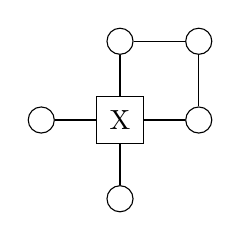
\begin{tikzpicture}[baseline=0.5]

                    \def \legLength { 0.8}
                    \def \radius {0.1}

                    \pgfmathsetmacro{\step}{2*\radius+ \legLength} % 1
                    \pgfmathsetmacro{\legpos}{\radius+\legLength} %0.9

                    \node[draw, circle,radius=\radius] (L0) at (-1,0) {};

                    \draw (-0.3,0.3) -- (0.3,0.3) -- (0.3,-0.3) -- (-0.3,-0.3) -- cycle;

                    \node[draw, circle,radius=\radius] (R0) at (1,0) {};
                    \node[draw, circle,radius=\radius] (R1) at (1,1) {};

                    \node[draw, circle,radius=\radius] (U) at (0,1) {};
                    \node[draw, circle,radius=\radius] (D) at (0,-1) {};

                    \draw (R0) --   (R1);

                    \draw (L0) --   (-0.3,0);

                    \draw (R0) --   (0.3,0);
                    \draw (U) --   (0,0.3);
                    \draw (D) --   (0,-0.3);
                    \draw (R1) --   (U);

                    \node[draw=none] (C0) at (0,0) {X};
                \end{tikzpicture} }}
    \end{equation}
\end{frame}

\def \figa { \vcenter{\hbox{ \pepob{5}{3}{{
                        "","","","",
                        "","","","",
                        "","","",""}}{{
                        "","",
                        "","",
                        "","",
                        "","",
                        "",""}}{{
                        1,1,1,1,1,
                        1,0,0,0,1,
                        1,0,0,0,1}} } }}

\def \figb { \vcenter{\hbox{  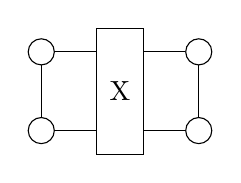
\begin{tikzpicture}[baseline=0.5]

                \def \legLength { 0.8}
                \def \radius {0.1}

                \pgfmathsetmacro{\step}{2*\radius+ \legLength} % 1
                \pgfmathsetmacro{\legpos}{\radius+\legLength} %0.9

                \node[draw, circle,radius=\radius] (L0) at (-1,0) {};
                \node[draw, circle,radius=\radius] (L1) at (-1,1) {};

                \draw (-0.3,1.3) -- (0.3,1.3) -- (0.3,-0.3) -- (-0.3,-0.3) -- cycle;

                \node[draw, circle,radius=\radius] (R0) at (1,0) {};
                \node[draw, circle,radius=\radius] (R1) at (1,1) {};

                \draw (L0) --   (L1);
                \draw (R0) --   (R1);

                \draw (L0) --   (-0.3,0);
                \draw (L1) --   (-0.3,1);

                \draw (R0) --   (0.3,0);
                \draw (R1) --   (0.3,1);

                \node[draw=none] (C0) at (0,0.5) {X};
            \end{tikzpicture}}}}

\def \figc {\vcenter{\hbox{  \begin{tikzpicture}[baseline=0.5]

                \def \legLength { 0.8}
                \def \radius {0.1}

                \pgfmathsetmacro{\step}{2*\radius+ \legLength} % 1
                \pgfmathsetmacro{\legpos}{\radius+\legLength} %0.9

                \node[draw=none, circle,radius=\radius] (L0) at (-1,0) {};
                \node[draw=none, circle,radius=\radius] (L1) at (-1,1) {};

                \draw (-0.3,1.3) -- (0.3,1.3) -- (0.3,-0.3) -- (-0.3,-0.3) -- cycle;

                \node[draw=none, circle,radius=\radius] (R0) at (1,0) {};
                \node[draw=none, circle,radius=\radius] (R1) at (1,1) {};

                \draw (L0) --   (-0.3,0);
                \draw (L1) --   (-0.3,1);

                \draw (R0) --   (0.3,0);
                \draw (R1) --   (0.3,1);

                \node[draw=none] (C0) at (0,0.5) {X};
            \end{tikzpicture} }} }

\def \figd {\vcenter{\hbox{  \begin{tikzpicture}[baseline=0.5]

                \def \legLength { 0.8}
                \def \radius {0.1}

                \pgfmathsetmacro{\step}{2*\radius+ \legLength} % 1
                \pgfmathsetmacro{\legpos}{\radius+\legLength} %0.9

                \node[draw=none, circle,radius=\radius] (L0) at (-1,0) {};
                \node[draw=none, circle,radius=\radius] (L1) at (-1,1) {};

                \node[draw, circle,radius=\radius] (C0) at (0,0) {};
                \node[draw, circle,radius=\radius] (C1) at (0,1) {};

                \node[draw=none, circle,radius=\radius] (R0) at (1,0) {};
                \node[draw=none, circle,radius=\radius] (R1) at (1,1) {};

                \draw (L0) --   (C0);
                \draw (L1) --   (C1);

                \draw (R0) --   (C0);
                \draw (R1) --   (C1);

                \draw (C1) --   (C0);
            \end{tikzpicture} }}}

\begin{frame}{Linear Solver: Applicability}
    \begin{equation}
        \figa
    \end{equation}

    \begin{subequations}
        \begin{align}
             & \figb          \\
             & \figc =  \figd
        \end{align}
    \end{subequations}
\end{frame}

\subsection{Nonlinear Solver}
\begin{frame}{Nonlinear Solver}
    \begin{itemize}
        \item Nonlinear least squares
        \item Jacobian
        \item Permutations
    \end{itemize}
\end{frame}

\subsection{Sequential Linear Solver}
\begin{frame}{Sequential Linear Solver}
    \begin{itemize}
        \item Based on linear solver
        \item Sweep over unknown tensors
        \item Permutations
    \end{itemize}
\end{frame}